\section{Fixed Pattern Noise}
\label{chap:patternnoise}

\def\hdrlfpn{{\em hdrl\_fpn}}

The pattern noise (PN, hereafter) is an almost regular pattern that 
appears on the images. Most likely it is due to electronic 
interference. Perhaps, the simplest PN example is the odd-even 
column/row effect -- a pattern in which consecutive
columns/rows  
have systematically different levels. 
Despite being called {\bf fixed}, the PN is transient and can vary
significantly between frames  of a sequence.

The PN not easily detectable by simple visual image inspection: a 
``good'' image (Fig. \ref{fig:patternnoise_non_diff}, left) is not 
much different from a ``bad'' image (Fig. \ref{fig:patternnoise_non_diff}, 
right), because the amplitude of the pattern may easily be smaller 
than the random noise level. In the special case when the pattern 
is aligned along the columns/rows, compacting the image in the 
direction of alignment can help to make the PN visible, but this 
is not the possible in general.

\begin{figure}[H]
  \centering \subfigure
  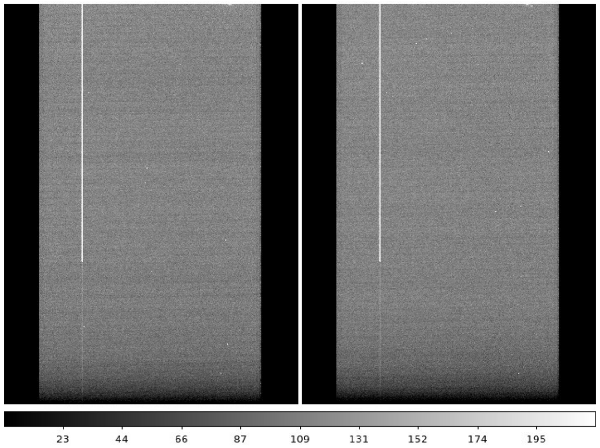
\includegraphics[width=10.0cm]{figures/patternnoise_non-diff.png} 
  \caption[]{\footnotesize Raw GIRAFFE bias images. The vertical stripe 
  is a detector artifact. Here and in the next figures, except for 
  Fig. \ref{fig:patternnoise_test_image}, the left and the right panels 
  use the same stretch to facilitate easier comparison. Here and further 
  the units are ADU.}
  \label{fig:patternnoise_non_diff}
\end{figure}

Fortunately, the PN shows prominently as a set of structures in the power 
spectra. The power spectrum of an ideal image, without any 
pattern, is a perfect delta function with a width of one pixel
(Fig. \ref{fig:patternnoise_test_image}).
The power concentrated in that single peak reflects the simple 
pixel-to-pixel sensitivity variation that is corrected by flat 
fielding. 
Other peaks and structures in the power spectrum indicate the 
presence of systematic noises, e.g. patterns.

However, if the analysed image is a science frame
and contains astronomical objects, these objects themselves will 
introduce peaks in the power spectrum that correspond to variations
on the scales of these objects. Therefore, the search for PN should
be performed on calibration frames, e.g. biases.

The function described here calculates the 2D power spectrum of an
input image, then masks a region around the peak corresponding to
the pixel-to-pixel variations, and then calculates on the remaining 
area of the power spectrum the root mean square (RMS) and the 
mean-absolute-deviation (MAD). A high RMS indicates the presence of
power in variations of any spatial scale and type of PN. The MAD is 
used as a reference level -- it indicates the typical level of the 
random variations of any scale. 

Summarizing, the advantage of this diagnostics is that 
it is sensitive to the PN of any spatial scale or spatial pattern type,
and it is not sensitive to the pixel-to-pixel variations.

\begin{figure}[H]
  \centering \subfigure
  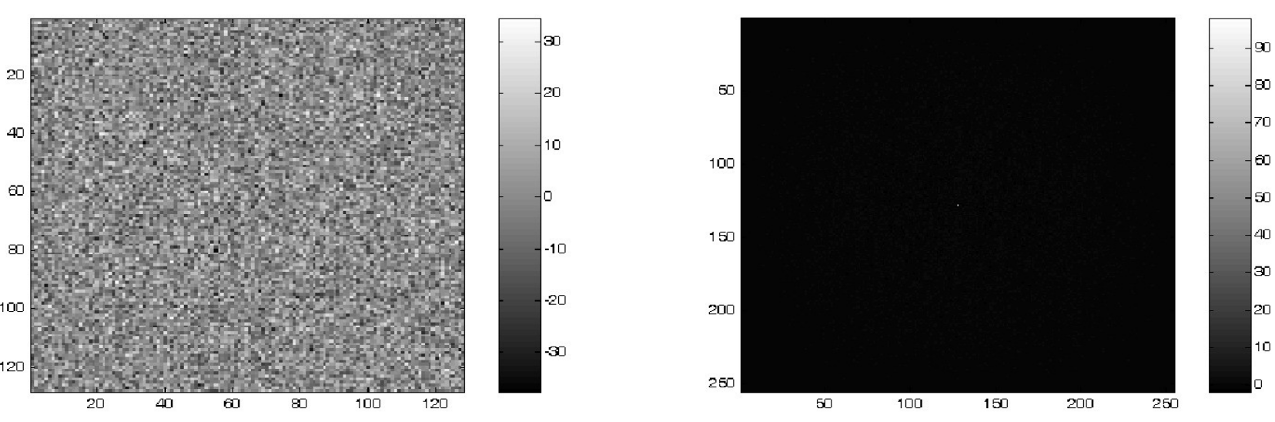
\includegraphics[width=12.0cm]{figures/patternnoise_test-image.png} 
  \caption[]{\footnotesize  {\bf Left Panel:}  Random noise image 
  with no patterns. \\
    {\bf Right Panel:} Its power spectrum (delta function at the centre). }
  \label{fig:patternnoise_test_image}
\end{figure}

Disclaimer: if the described power spectrum 
analysis is applied directly on real raw data, it may be 
affected by any structures such as cosmetic defects (e.g. bad 
columns/areas) and count decrease at the edges (e.g. due to 
vignetting). These changes are systematic in nature and they will 
show prominently in the power spectra, making the signatures 
of the transient PN almost invisible 
(Fig. \ref{fig:patternnoise_giraffe_image}).

\begin{figure}[H]
  \centering \subfigure
  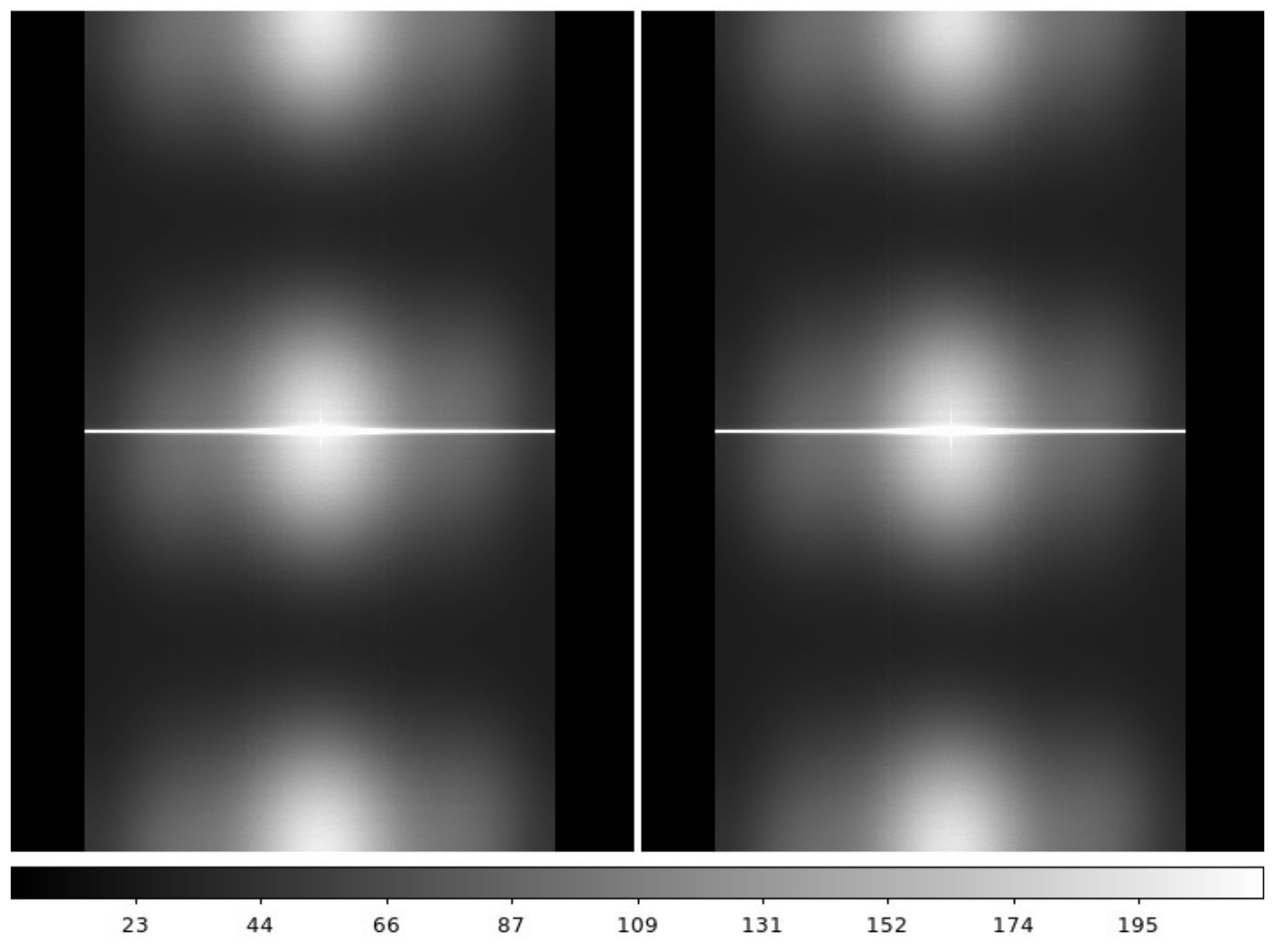
\includegraphics[width=10.0cm]{figures/patternnoise_giraffe-image.png} 
  \caption[]{\footnotesize Power spectra of the raw GIRAFFE bias images.}
  \label{fig:patternnoise_giraffe_image}
\end{figure}

Therefore, some pre-reduction may be necessary: removing the large 
artefacts from the images, repairing the cosmic rays (in our case -- 
replacing the affected pixels with averages from their neighbours), 
and taking out any stable known global patterns like any permanent 
gradients in the illumination or bias level. 
Figure \ref{fig:patternnoise_giraffe_repair_bias} shows an example 
of a ``repaired'' GIRAFFE images).

\begin{figure}[H]
  \centering \subfigure
  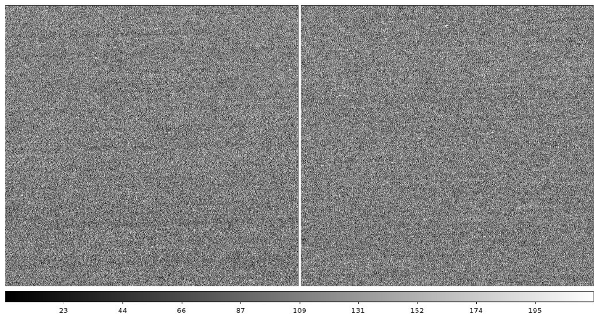
\includegraphics[width=12.0cm]{figures/patternnoise_giraffe-repair_bias.png} 
  \caption[]{\footnotesize ``Repaired'' GIRAFFE bias images.}
  \label{fig:patternnoise_giraffe_repair_bias}
\end{figure}

The power spectra of the ``repaired'' images shows great improvement 
as seen in Fig. \ref{fig:patternnoise_giraffe_repair_powerSpectra} --
compare the weak power present on the left image, and strong power on 
the right image.

The time scale of the PN variations must also be taken into account in this 
analysis, especially if one wants to apply the detection algorithm on 
combined master frames of some kind, e.g. on master biases. If the 
PN varies too quickly, the combination into master bias will average 
over many different types of PN and the resulting image will be 
unrealistically ``clean''. In such cases the analysis should be 
carried out on individual raw images. It is important to investigate 
the PN variation time scale before adopting a procedure for a 
particular instrument/detector.


\begin{figure}[H]
  \centering \subfigure
  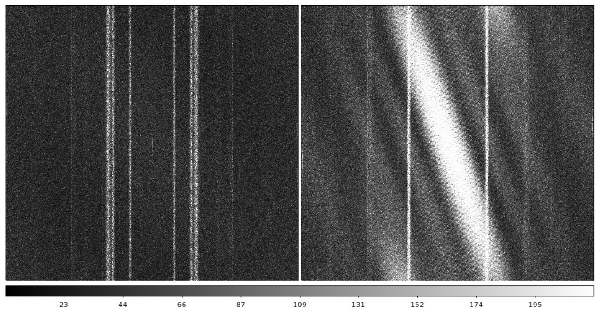
\includegraphics[width=12.0cm]{figures/patternnoise_giraffe-repair_powerSpectra.png} 
  \caption[]{\footnotesize Power spectra of the ``repaired'' GIRAFFE bias. 
  The image on the left shows no pattern noise, the image on the right is 
  affected by pattern noise.}
  \label{fig:patternnoise_giraffe_repair_powerSpectra}
\end{figure}

% To quantify the presence of pattern noise we propose a simple quality 
% control (QC) parameter: fraction of the pixels in the power spectrum that 
% exceed a certain limit. 
% Figure \ref{fig:patternnoise_giraffe_repair_histogram} shows a histogram 
% of this fraction from processing 195 GIRAFFE bias images extracted from 
% the ESO science archive. The adopted limit here was 30 ADU. This limit 
% depends on the instrument detector and the level of removal of any 
% permanent patterns; it must be derived empirically from the data. The 
% images with no pattern noise cluster in the peak centered at a fraction 
% $\sim 0.012 \%$, while the affected images cluster in the peak centered 
% at a fraction $\sim 0.06\%$. A comparison of the top (for not pre-reduced 
% images) and bottom (for reduced images) panels shows that the cleaning of 
% bad columns and pixels improves the separation between the ``good'' and 
% the ``bad'' images. The peak of the affected images is broader, indicating 
% that the pattern noise varies from one image to another.
% 
% 
% \begin{figure}[H]
%   \centering \subfigure
%   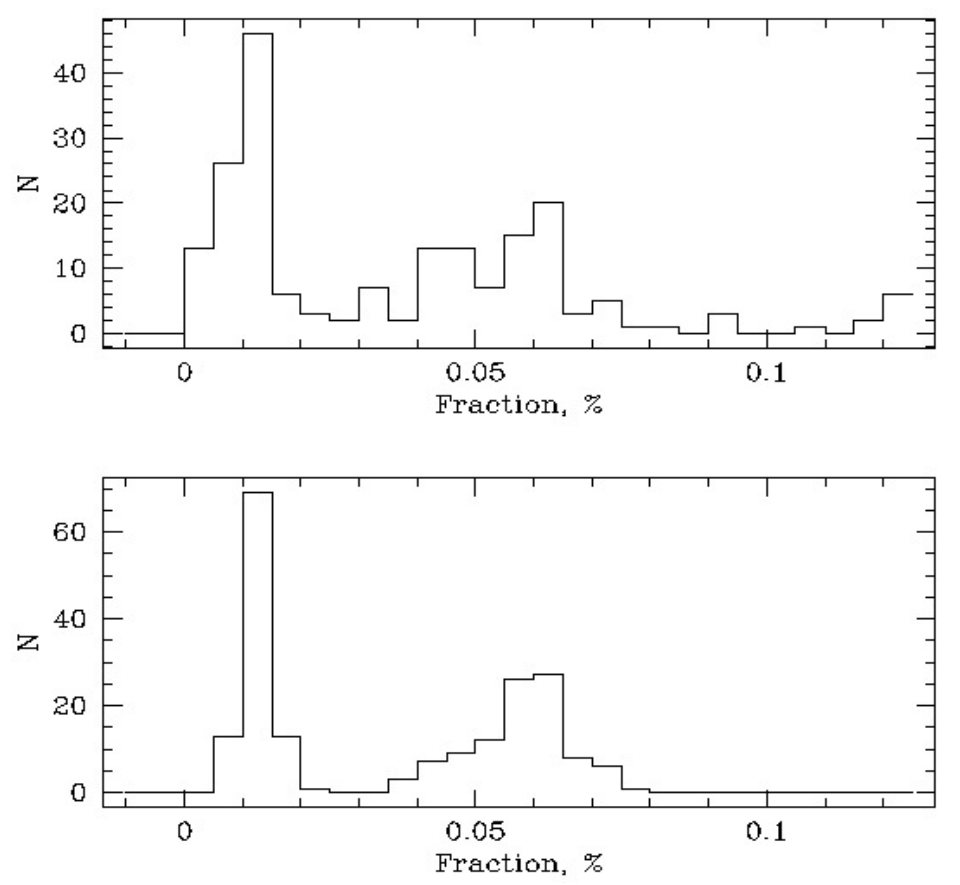
\includegraphics[width=10.0cm]{figures/patternnoise_giraffe-repair_histogram.png} 
%   \caption[]{\footnotesize Histogram of the fraction of pixels (in percent) 
%   above the adopted limit for GIRAFFE raw (top) and ``repaired'' (bottom) 
%   bias images.}
%   \label{fig:patternnoise_giraffe_repair_histogram}
% \end{figure}
